\chapter{Requirements}

\section{Functional requirements}
The following requirements have been elicited with respect to the domain properties and assumptions mentioned above in order to satisfy the goals.

\subsection{Basic requirements}
\begin{itemize}
	\item \ref{goal:registration} \refitemtext{goal:registration}:
	\begin{itemize}
		\item The system needs to provide mandatory sign up and payment options for the guest users who wants to register to use the car sharing service.
		\item Once the payment is successful and the guest user is registered, the registered user receives a password that can be used to access (login into) the system.
	\end{itemize}

	\item \ref{goal:cars_location} \refitemtext{goal:cars_location}:
	\begin{itemize}
		\item The system needs to provide the exact location of the cars that are available within a certain distance either from the current location of the registered users or from a specified address given(entered) by the registered users.
	\end{itemize}

	\item \ref{goal:reservation} \refitemtext{goal:reservation}:
	\begin{itemize}
		\item The system provides provision such that the registered users must be able to reserve only a single car among the available cars in a certain geographical region for up to one hour before they pick it up.
	\end{itemize}

	\item \ref{goal:expiration} \refitemtext{goal:expiration}:
	\begin{itemize}
		\item The system checks if a reserved car is picked-up within one hour.
		\item If not, the system tags the car as available again and the reservation expires.
		\item The system penalizes the registered user who made the reservation and did not pick the reserved car within an hour, by making him to pay a fee of \EUR{1}.
	\end{itemize}

	\item \ref{goal:entry} \refitemtext{goal:entry}:
	\begin{itemize}
		\item The system must be able to identify (communicate with) the registered user when he/she is nearby the reserved car.
		\item The system unlocks the reserved car and allows the registered user to enter it after identification of registered user as mentioned in the previous point.
	\end{itemize}

	\item \ref{goal:charging} \refitemtext{goal:charging}:
	\begin{itemize}
		\item The system starts charging the registered user for a given amount of money per minute as soon as the engine is ignited.
		\item The system must be able to notify the current charges to the registered user through a screen on the reserved car.
	\end{itemize}

	\item \ref{goal:car_locking} \refitemtext{goal:car_locking}:
	\begin{itemize}
		\item The system must stop charging the registered user as soon as the reserved car is parked in a safe area and the registered user exits the reserved car.
		\item The system must be able to lock the reserved car automatically at this point after the above operation is successfully done.
	\end{itemize}

	\item \ref{goal:safe_areas} \refitemtext{goal:safe_areas}: \\ The safe areas are defined by the systems as follows:
	\begin{itemize}
		\item Those areas predefined by the system in and around a specific geographical region (green areas displayed in the user interface screen)
		\item The parking areas which are not private and located in the basement (underground).
		\item The parking area in which the GPS signals are not very low (the system must suggest the user in this case).
	\end{itemize}
\end{itemize}

\subsection{Value added requirements}
In addition to the above requirements, the system should motivate the virtuous behaviors of the registered user by satisfying the following requirements:

\begin{itemize}
	\item \ref{goal:passengers} \refitemtext{goal:passengers}:
	\begin{itemize}
		\item The system must detect if the registered user has taken at least two other passengers onto the reserved car. 
		\item The system must calculate and apply a discount of 10\% on the last ride if the above-mentioned point is true or satisfied.
	\end{itemize}

	\item \ref{goal:battery} \refitemtext{goal:battery}:
	\begin{itemize}
		\item The system must detect the percentage of the battery charge that has been consumed in the reserved car by the registered user during the last ride.
		\item The system must calculate and apply a discount of 20\% if the reserved car is left with no more than 50\% of the battery empty.
	\end{itemize}

	\item \ref{goal:special_areas} \refitemtext{goal:special_areas}:
	\begin{itemize}
		\item The system should detect if the reserved car is left in the special parking areas-where they can be recharged and the registered user takes care of plugging the car into the power grid.
		\item The system must calculate and apply a discount of 30\% on the last ride if the above check is true or satisfied.
	\end{itemize}

	\item \ref{goal:constraints} \refitemtext{goal:constraints}: \\ The system must check if either of the following conditions are true:
	\begin{itemize}
		\item The distance between the reserved car (parked after the ride) and the nearest power grid station is more than 3KM (Kilometers).
		\item The battery of the reserved car (parked after the ride) is consumed more than 80\%.
		\item The system must penalize the registered user by charging 30\% more on the last ride if either of the two conditions mentioned above are true to compensate for the cost required to recharge the reserved car (parked after the ride).
	\end{itemize}
\end{itemize}

\subsection{Operations allowed to users}
We have clearly elicited the requirements of PowerEnJoy for which the functional requirements are stated as follows:
\begin{itemize}
	\item \emph{Guest user}:
	\begin{itemize}
		\item Sign up.
	\end{itemize}

	\item \emph{Registered user}:
	\begin{itemize}
		\item Login.
		\item Find the location of available cars.
		\item Select his/her final destination.
		\item Reserve an available car.
		\item Receive notification of the reservation expiry and penalty.
		\item Enter the reserved car (by communicating with the system).
		\item Receive notification of the current charges.
		\item Park the reserved car in safe areas.
		\item Take at least two other passengers onto the reserved car and avail discount.
		\item Minimize the consumption of the battery's charge in the reserved car to avail discount.
		\item Park the reserved car in special parking areas and avail discount.
		\item Select (Enable) the money saving option to get discount.
	\end{itemize}
\end{itemize}

\section{Non-functional requirements}

\subsection{User interface}
The user interface of our application is thought to be used via web as well as a mobile application. There are two sketches of the UI screen which are displayed below.

\begin{figure}[t]
	\centering
	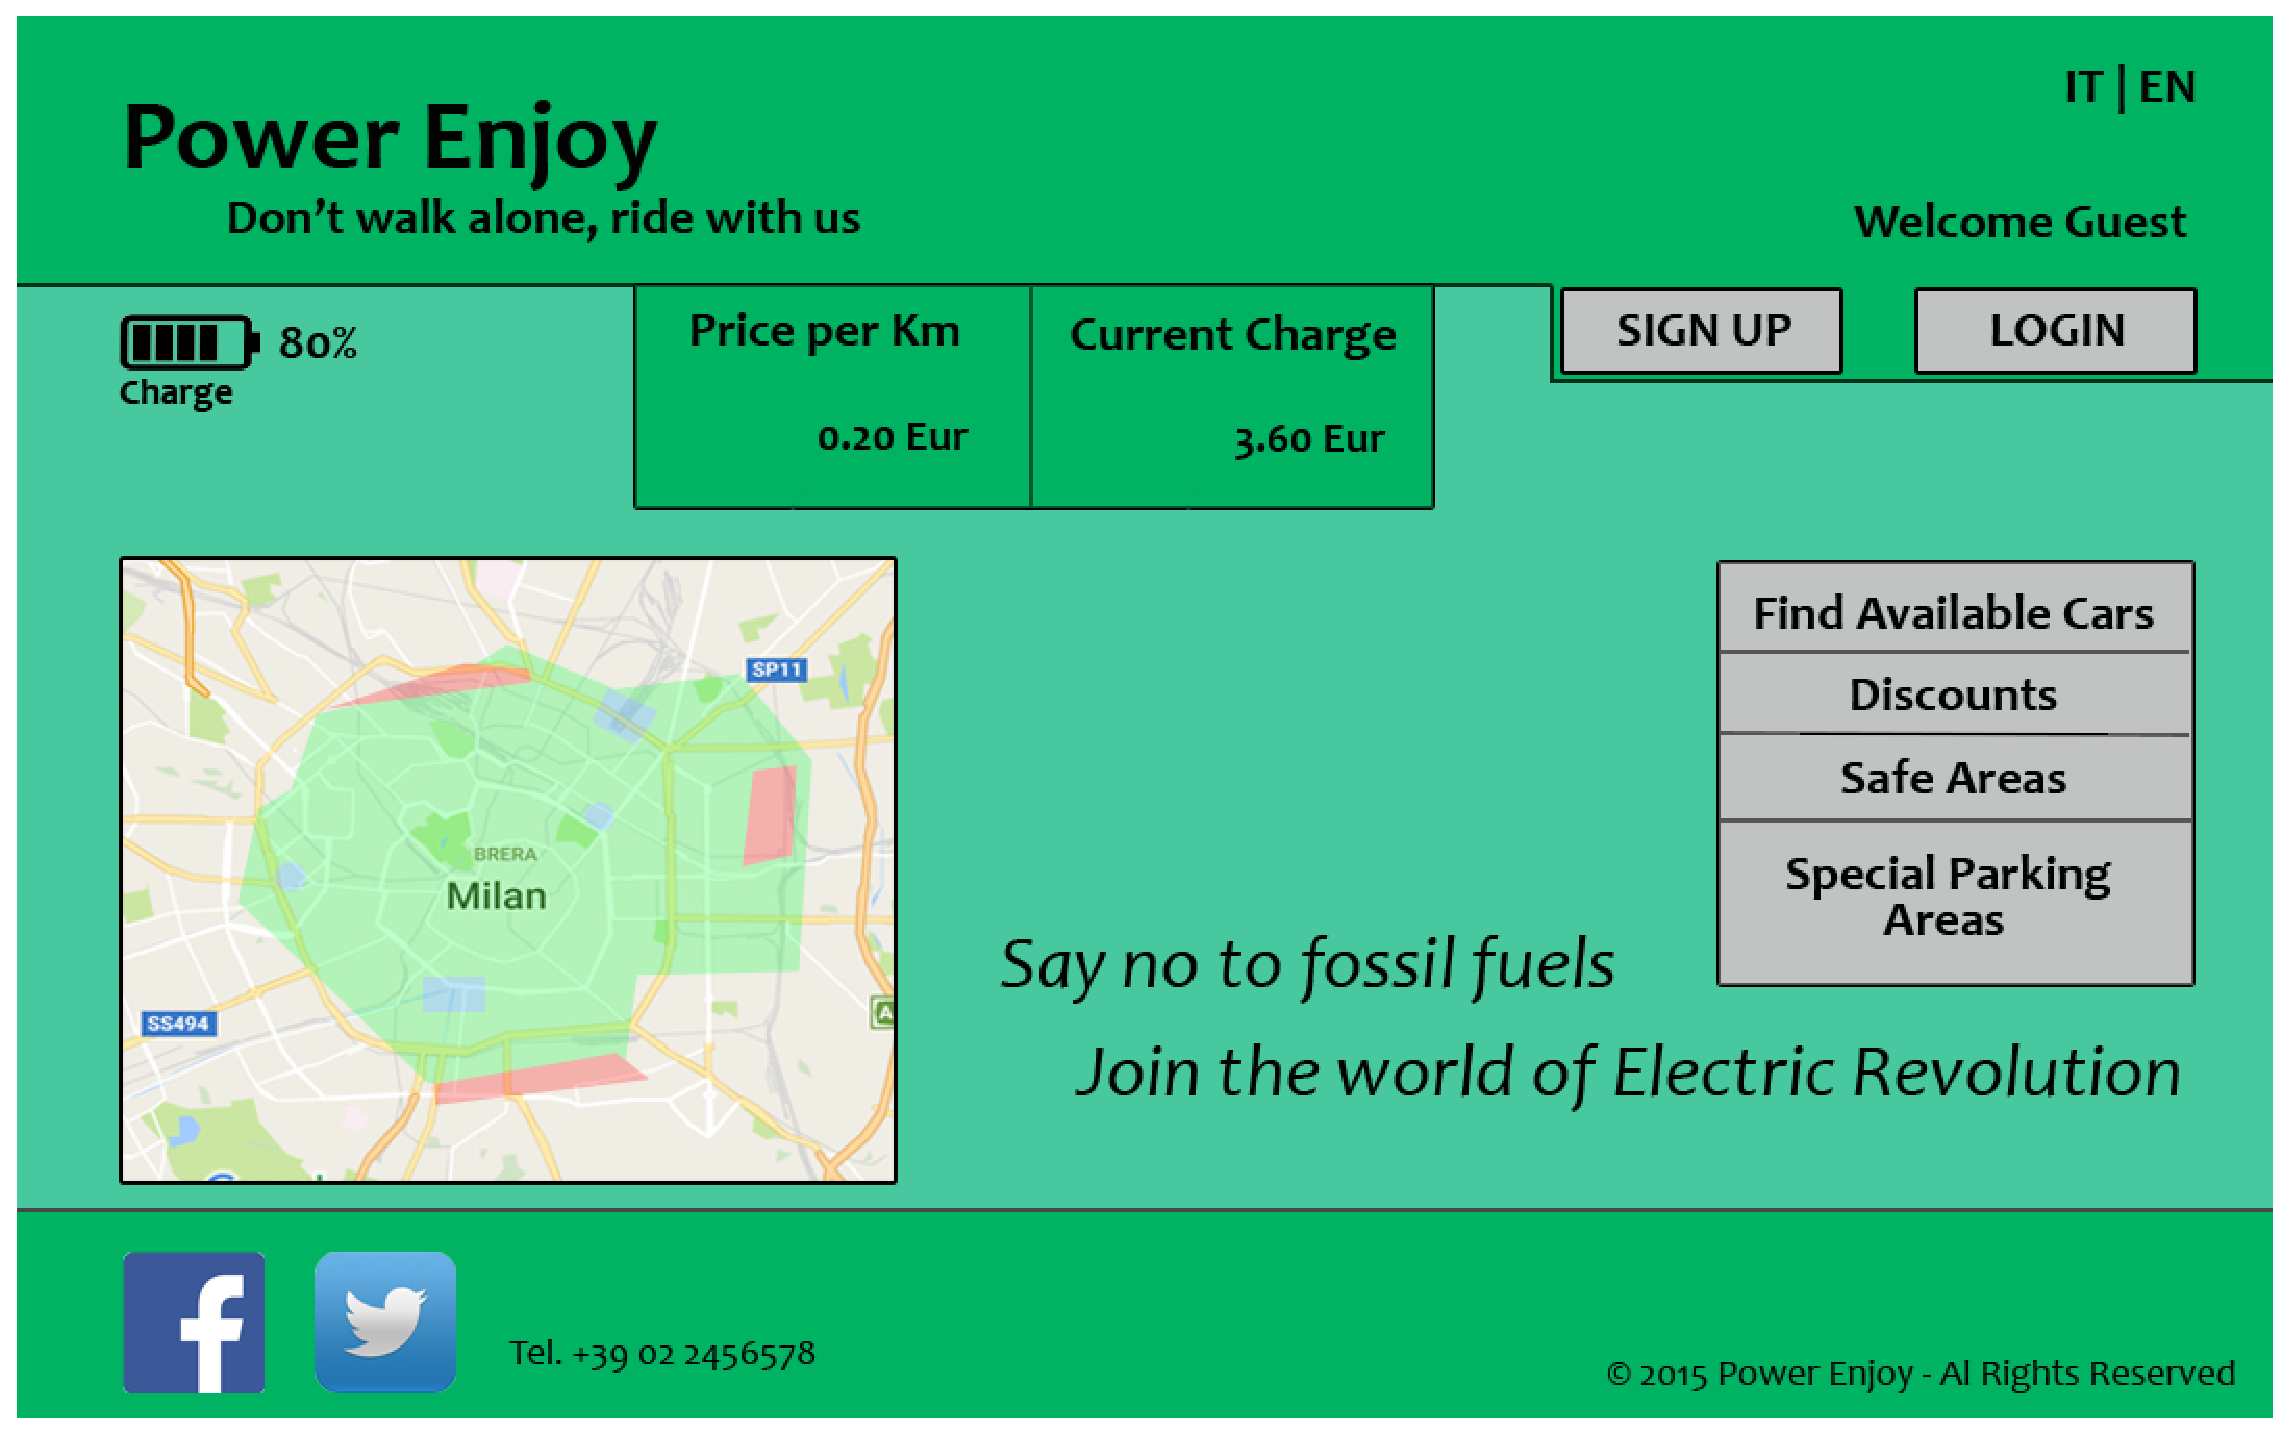
\includegraphics[height=8cm,keepaspectratio]{figures/desktop.eps}
	\caption{Desktop UI of PowerEnJoy login page}
	\label{fig:desktop}
\end{figure}

The figure~\ref{fig:desktop} shows the homepage that any guest user can see. It displays the sign up and login option; options like finding available cars, reserving an available car, money saving option, charge per km with current charge, homepage page of the desktop version.

\begin{figure}[t]
	\centering
	\begin{minipage}{0.45\textwidth}
		\centering
		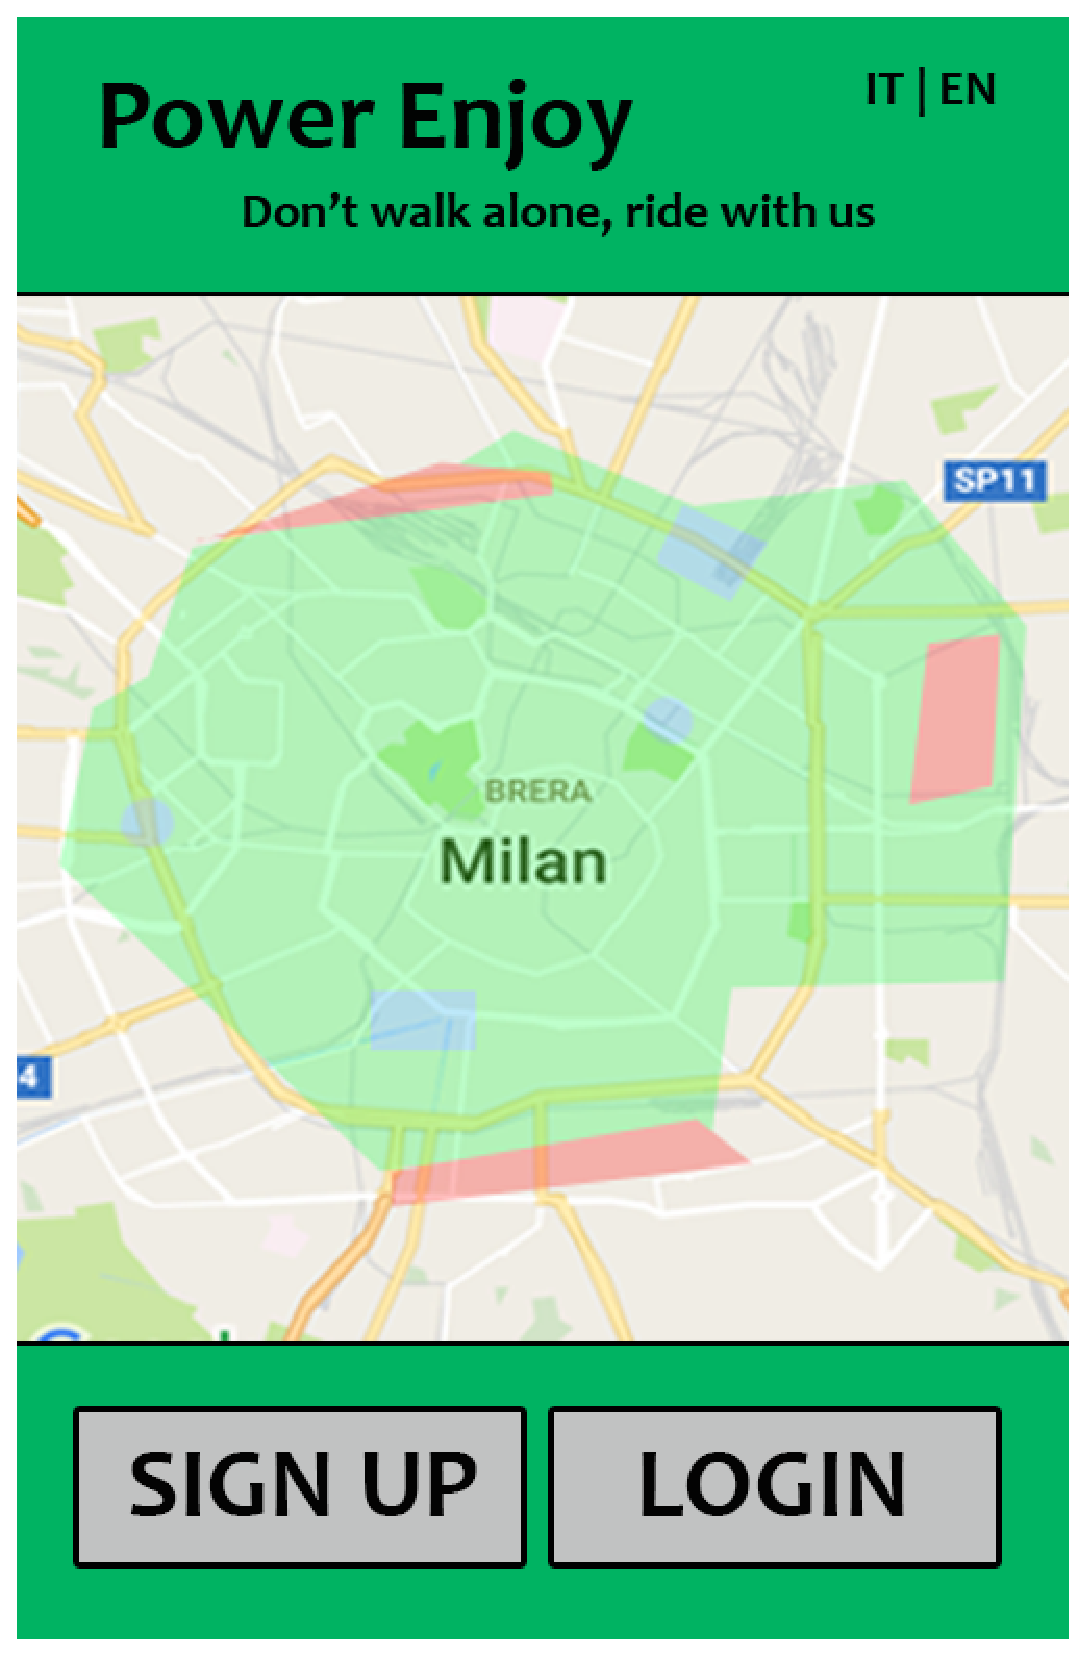
\includegraphics[width=0.9\textwidth]{figures/mobile.eps} % first figure itself
		\caption{Mobile UI of PowerEnJoy login page}
		\label{fig:mobile}
	\end{minipage}\hfill
	\begin{minipage}{0.45\textwidth}
		\centering
		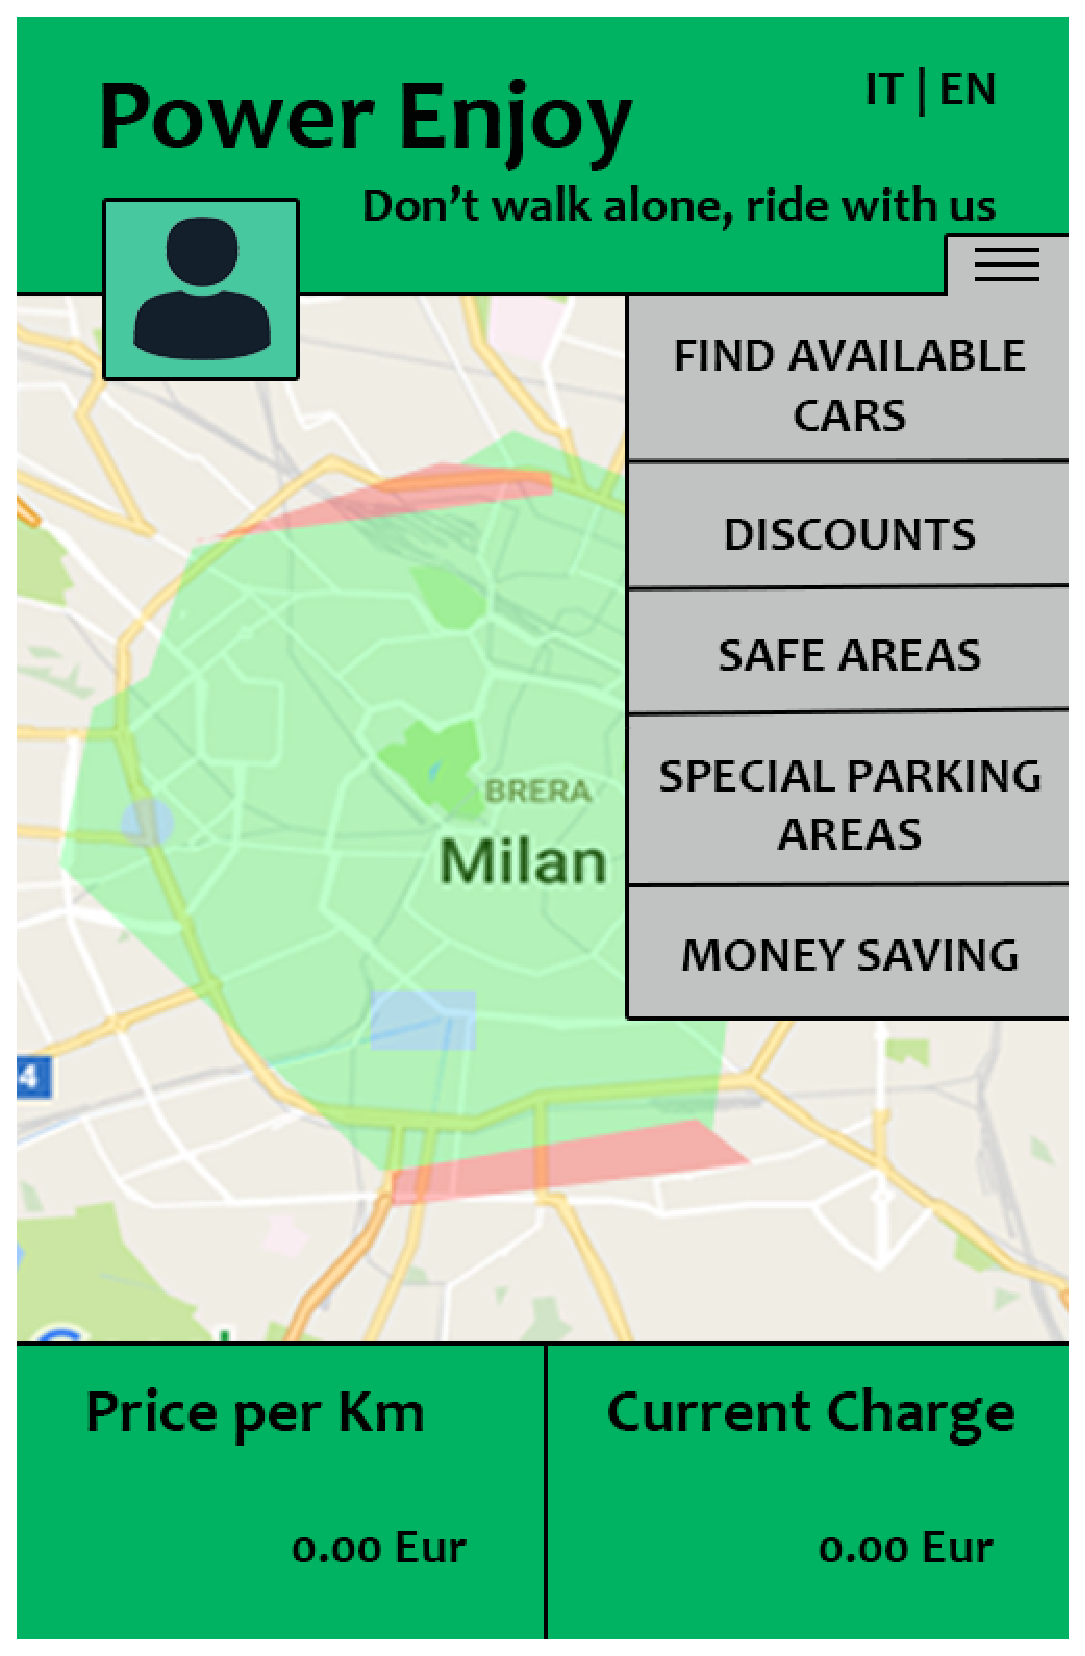
\includegraphics[width=0.9\textwidth]{figures/mobile_logged.eps}
		\caption{Mobile UI of PowerEnJoy homepage}
		\label{fig:mobile_logged}
	\end{minipage}
\end{figure}

The figure~\ref{fig:mobile} shows the features and option in a mobile application. The first picture in the below area shows the HOME page of the application before login. It shows the sign up and login option for the guest user. It also displays the availability of cars in nearby area through GPS.

The figure~\ref{fig:mobile_logged} displays the screen after a registered user logins. It has options like: find the available cars, reserve a car, discounts, safe area,	special parking areas, money saving option, price per km with current charge.

\subsection{Documentation}
We will release the following documents in order to organize our work in each phase of the development process and keep in touch with the stakeholders.
\begin{itemize}
	\item RASD, Requirement Analysis and Specification Document, which defines our goals and assumptions and contains an overall description of the system (using scenarios and use-cases) and the models describing requirements and specifications.
	\item DD, Design Document, which contains a functional description of the system using models such as UML diagrams.
	\item Installation manual, which explains how to deploy the web site.
	\item User manual, which explains users how to use the main functionalities of the web site.
	\item Testing report, which contains the results of the testing activity performed on a system developed by another group.
	\item Project reporting, which is the result of some analysis done on the project activity.
\end{itemize}